%*****************************************
\chapter{Alethe: A New Standard for Proof Trace Representation}\label{ch:alethe}
%*****************************************

\section{The Alethe Proof Format}

Alethe \cite{alethe,alethe2} is a modern proof format for SMT, designed to facilitate integration with proof assistants.
It has been co-developed with proof checkers in Isabelle/HOL \cite{aletheInIsa} and currently supports proofs in the theories of uninterpreted functions (\textbf{UF}), linear arithmetic (\textbf{LA}), and linear integer arithmetic (\textbf{LIA}), while support for bit-vectors (\textbf{BV}) is under active development.
As a result, for SMT fragments covered by Alethe, solver results can be verified inside proof assistants to prove correction of the solver.

The format is intended as a flexible and uniform representation of \emph{unsatisfiability} proofs produced by SMT solvers as described in \cref{sec:smt-proof}.
Its design combines a natural-deduction style structure with a set of rules operating on first-order clauses.
The language of Alethe is based on SMT-LIB \cite{smtlib}, and therefore inherits its many-sorted first-order logic as foundation base.
With the exception of clauses for propositional reasoning, there is no dedicated syntax for any theory.

Beyond serving as an interchange format, Alethe aims to keep proofs accessible to both humans and automated tools.
Proofs are intended to be readable by humans, easily checked, and readily consumable by other systems such as interactive theorem provers or stand-alone proof checkers \cite{carcara}.
The format is already adopted in practice, being supported by the SMT solvers veriT \cite{verit} and cvc5 \cite{cvc5}, and ongoing development for the Constrained Horn Clauses solver Golem \cite{golem}.

\section{The Alethe Language}

The Alethe proof trace format \cite{alethespec} for SMT solvers comprises two parts: the trace language based on SMT-LIB and a collection of proof rules. Traces witness proofs of unsatisfiability of a set of constraints.
They are sequences $a_1 \dots a_m~t_1 \dots t_n$ where
the $a_i$ corresponds to the constraints of the original SMT problem being refuted, each $t_i$ is a clause inferred from previous elements of the sequence, and $t_n$ is $\bot$ (the empty clause).
In the following, we designate the SMT-LIB problem as the \emph{input problem}.

\begin{lstlisting}[language=SMT]
(set-logic UF)
(declare-sort U 0)
(declare-fun a () U)
(declare-fun b () U)
(declare-fun p (U) Bool)
(assert (p a))
(assert (= a b))
(assert (not (p b)))
(check-sat)
(get-proof)
\end{lstlisting}

\begin{center}
$\lightning$
\end{center}

\begin{lstlisting}[language=SMT,caption={Running example: an SMT problem and its Alethe proof found by cvc5.},label={lst:smtexampleinput-fol}]
(assume a0 (p a))
(assume a1 (= a b))
(assume a2 (not (p b)))
(step t1 (cl (not (= (p a) (p b))) (not (p a)) (p b)) :rule equiv_pos2)
(step t2 (cl (= (p a) (p b))) :rule cong :premises (a1))
(step t3 (cl (p b)) :rule resolution :premises (t1 t2 a0))
(step t4 (cl) :rule resolution :premises (a2 t3))
\end{lstlisting}


We will use the input problem shown in the top part of \cref{lst:smtexampleinput-fol} with its Alethe proof (found by cvc5) in the bottom part as a running example (for \textbf{UF} logic) to provide an overview of Alethe concepts and to illustrate our embedding in Lambdapi.
The \emph{input problem} is given as a script consisting of commands that interact with the SMT solver.
For example, in \cref{lst:smtexampleinput-fol}, \smtinline{assert} introduces an assertion, \smtinline{check-sat} triggers the solving process, and \smtinline{get-proof} requests the solver to output a proof.
In the following, we introduce the concepts needed to understand the proof produced by cvc5 in \cref{lst:smtexampleinput-fol}.

\subsection{Many-Sorted First-Order Logic}

An Alethe proof trace inherits the declarations of its input problem. All symbols (sorts, functions, assertions, etc.) declared or defined in the input problem remain declared or defined, respectively.
Furthermore, the syntax for terms, sorts, and annotations uses the syntactic rules defined in SMT-LIB \cite[\S 3]{smtlib} and the SMT signature context defined in \cite[\S 5.1 and \S 5.2]{smtlib}.
The set of sorts present in a proof depends on the chosen SMT-LIB logic or theory, in addition to any sorts introduced by the user.
However, the sort \smtinline{Bool} is always included.

Alethe extends the SMT-LIB with Hilbert's choice operator $\epsilon$ (\smtinline{choice} in ASCII). A term of the form $\epsilon x.\,P(x)$ denotes a witness $\nu$ such that $P(\nu)$ holds if such a witness exists; if not, the term denotes an arbitrary value.
To ensure coherence, Alethe enforces functionality of the choice operator with respect to logical equivalence: for any formulas $P$ and $Q$ with free variable $x$, if $\forall x.\,P \simeq Q$, then it must also hold that $\epsilon\, x.\,P \simeq \epsilon\, x.\,Q$.

\subsection{Steps}

An Alethe proof is represented as an indexed sequence of steps.
In order to reflect the concrete syntax of Alethe proofs, we denote proof steps in the abstract notation by the following form:

\renewcommand{\eqnhighlightshade}{35}

\begin{equation}
\label{eq:step}
\tag{\textcolor{purple}{1}}
\eqnmarkbox[indexClr]{node2}{i}. \quad \eqnmarkbox[blue]{node1}{\Gamma} ~\triangleright~ \eqnmarkbox[green]{node3}{l_1 \dots l_n} \quad (\eqnmarkbox[purple]{node4}{\mathcal{R}}~\eqnmarkbox[red]{node5}{p_1 \dots p_m})~\eqnmarkbox[orange]{node6}{[a_1 \dots a_r]}
\end{equation}

\vspace{0.3em}
\annotate[yshift=-0.5em]{below, left}{node2}{index}
\annotate[yshift=-0.5em]{below, right}{node1}{context}
\annotate[yshift=0.5em]{above, left}{node3}{clause}
\annotate[yshift=-0.5em]{below, right}{node4}{rule}
\annotate[yshift=-0.5em]{below, right}{node5}{premises}
\annotate[yshift=-0.5em]{below, right}{node6}{arguments}

\vspace{0.3em}

\medskip

A step \cref{eq:step} consists of an index \colorbox{indexClr!30}{$i$} $\in \mathbb{I}$ where $\mathbb{I}$ is a countable infinite set of indices (e.g. \kw{a0}, \kw{t1}), and a clause of formulae \colorbox{green!30}{$l_1, \dots, l_n$} representing an $n$-ary disjunction. Steps that are not assumptions are justified by a proof rule \colorbox{purple!30}{$\mathcal{R}$} that depends on a possibly empty set of premises $\{\colorbox{red!30}{$p_1 \dots  p_m$}\} \subseteq \mathbb{I}$ that only references earlier steps such that the proof forms
a directed acyclic graph. A rule might also depend on a list of arguments \colorbox{orange!30}{$[a_1 \dots a_r]$} where each argument $a_i$ is either a term or a pair $(x_i, t_i)$ where $x_i$ is a variable and $t_i$ is a term. The interpretation of the arguments is rule specific. The context \colorbox{blue!30}{$\Gamma$} of a step is a list $c_1 \dots c_l $ where each element $c_j$ is either a variable or a variable-term tuple denoted $x_j \mapsto t_j$. Therefore, steps with a non-empty context contain variables $x_j$ that appear in \colorbox{green!30}{$l_i$} and will be substituted by $t_j$. Proof rules \colorbox{purple!30}{$\mathcal{R}$} include theory lemmas and \texttt{resolution}, which corresponds to hyper-resolution on ground first-order clauses.

We now have the key components to explain the guiding proof in the bottom part of \cref{lst:smtexampleinput-fol} that consists of seven steps. The proof starts with three \texttt{assume} steps \texttt{a0}, \texttt{a1}, \texttt{a2} that restate the assertions from the input problem.
In the concrete syntax, assume steps have a dedicated command \smtinline{assume} to clearly distinguish them from normal steps that use the \smtinline{step} command.
Step \texttt{t1} introduces a tautology of the form $\neg (\varphi_1 \approx \varphi_2) \lor \neg \varphi_1 \lor \varphi_2$, justified by the rule \colorbox{purple!30}{\texttt{equiv\_pos2}}. Steps \texttt{t2}, \texttt{t3}, \texttt{t4} use earlier premises that correspond to previous steps. Step \texttt{t2} proves $p(a) \approx p(b)$ by congruence (rule \colorbox{purple!30}{\texttt{cong}}) from the assumption \texttt{a1}.
Step \texttt{t3} applies the \colorbox{purple!30}{\texttt{resolution}} rule of propositional logic to the premises \texttt{t1, t2, a0} to derive $p(b)$. Finally, the step \texttt{t4} concludes the proof by generating the empty clause $\bot$, concretely denoted as \kw{(cl)} in \cref{lst:smtexampleinput-fol}. %(line 8)
Notice that the contexts \colorbox{blue!30}{$\Gamma$} of each step are all empty in this proof.

\subsection{Subproofs and Lemmas}
\label{ssec:subproof-desc}

Alethe uses subproofs to prove lemmas and to create and manipulate the context. To prove lemmas, a subproof can introduce
local assumptions. The \kw{subproof} use at step 2 in \cref{ex:subproof} discharges the local assumptions.
As the example shows, the abstract notation denotes subproofs by a frame around the steps in the subproof.
A subproof step cannot use a premise from a subproof nested within the current subproof.
Subproofs are also used to manipulate the context \colorbox{blue!30}{$\Gamma$}.

\begin{example}\label{ex:subproof}
This example shows a refutation of the formula $(2 + 2 ) \simeq 5$. The proof uses a subproof to prove the lemma $((2 + 2 ) \simeq 5) \implies 4 \simeq 5$.
Step 2 can be viewed as a lemma, and the steps $2.0 - 2.2$ are the intermediate steps to prove it.
\[
\begin{array}{r c l l}
1. & \triangleright & (2 + 2) \approx 5 & \text{assume} \\
\multicolumn{4}{l}{%
\begin{array}{r |r c l l}
& 2.0 & \triangleright & (2 + 2) \approx 5 & \text{assume} \\
& 2.1 & \triangleright & (2 + 2) \approx 4 & \text{sum\_simplify} \\
& 2.2 & \triangleright & 4 \approx 5 & \text{(trans 2, 3)} \\
\cline{2-5}
\end{array}
} \\
2. & \triangleright & \neg((2 + 2) \approx 5), 4 \approx 5 & \text{subproof} \\
3. & \triangleright & (4 \approx 5) \approx \bot & \text{eq\_simplify} \\
4. & \triangleright & \neg((4 \approx 5) \approx \bot), \neg(4 \approx 5), \bot & \text{equiv\_pos2} \\
5. & \triangleright & \bot & \text{(resolution 1, 2, 3, 4)}
\end{array}
\]
\end{example}

\subsubsection{Contexts}

Alethe contexts are a general mechanism to write substitutions and to change them by attaching new elements.
We recall that a context is a (possibly empty) list $c_1, \dots, c_n$, where each element $c_i$ is either:
\begin{enumerate}
  \item a variable $x_i$, called a \emph{fixing} of $x_i$, or
  \item a pair $x_i \mapsto t_i$, representing a substitution of $x_i$ by the term $t_i$.
\end{enumerate}

Every non-empty context $\Gamma$ induces a substitution $\mathop{subst}(\Gamma)$.
The induced substitution is always \emph{capture-avoiding}, i.e., it avoids binding free variables.

If $\Gamma$ ends with a fixing, the variable shadows any earlier substitution for it:
\[
\mathop{subst}([c_1, \dots, c_{n-1}, x_n]) \;=\;
\mathop{subst}([c_1, \dots, c_{n-1}]) \text{ with } x_n \mapsto x_n.
\]

If $\Gamma$ ends with a mapping, the substitution is extended accordingly:
\[
\mathop{subst}([c_1, \dots, c_{n-1}, x_n \mapsto t_n]) \;=\;
\mathop{subst}([c_1, \dots, c_{n-1}]) \circ \{x_n \mapsto t_n\},
\]
where $\circ$ denotes substitution composition.
The application of a context $\Gamma$ to a term $t$ is written $\mathop{subst}(\Gamma)(t)$.

\begin{example}
\begin{align*}
& \mathop{subst}([ x \mapsto 1, x \mapsto (g~x) ])(x)  = g(1) \\
& \mathop{subst}([ x \mapsto 1, x, x \mapsto (g~x)])(x) = g(x)
\end{align*}
\end{example}

Contexts are used to express proofs about the preprocessing of terms. The
conclusions of proof rules that use contexts always have the form

\begin{tabular}{l c r r}
i. & $\Gamma \quad \triangleright$ & $t \approx u$ & \kw{rule}... \\
\end{tabular}


where the term $t$ is the original term, and $u$ is the term after preprocessing. Tautologies with contexts correspond to judgments
$\models_\cal{T} \mathop{subst}(\Gamma)(t) \approx u$. Formally, the context is translated to $\lambda$-abstractions and applications \cite[\S 3.1]{alethespec}.

\begin{example}\label{ex:subproof-ctx}
Consider a subproof with the context $\Gamma = [y, x \mapsto y]$, used to rename a bound variable:
\[
\begin{array}{r c l l}
1. & \triangleright & \forall x, (P~x) & \kw{assume} \\
2. & \triangleright & \neg (\forall y, (P~y)) & \kw{assume} \\
\multicolumn{4}{l}{%
\begin{array}{r |r c l l}
& 3.0 & y, x \mapsto y~\triangleright & x \simeq y & \kw{assume} \\
& 3.1 & y, x \mapsto y~\triangleright & (P~x) \simeq (P~y) & \kw{cong}~3.0 \\
\cline{2-5}
\end{array}
} \\
3. & \triangleright & \forall x, (P~x) \simeq \forall y, (P~y) & \kw{bind} \\
4. & \triangleright & \neg(\forall x, (P~x) \simeq \forall y, (P~y)) & \\
  & \triangleright & \neg  \forall x, (P~x),  \forall y, (P~y) & \kw{equiv\_pos2} \\

5. & \triangleright & \bot & \kw{(resolution)~1\,2\,3\,4}
\end{array}
\]
In this case, the subproof concludes with a step that does not use the subproof rule, but another rule, such as the bind rule.
\end{example}

\begin{remark}
This kind of subproof in \cref{ex:subproof-ctx} is needed in Alethe to justify variable renaming under binders.
It is not relevant in Lambdapi, since Lambdapi relies on $\alpha$-equivalence when comparing terms with binders,
and therefore treats $\Pi\,x.\,P(x)$ and $\Pi\,y.\,P(y)$ as definitionally equal without requiring an explicit proof step.
\end{remark}

\section{The concrete syntax of Alethe}

We recall that the concrete ASCII representation of the Alethe proofs is based on the SMT-LIB standard.
\cref{fig:syntax-alethe-example} shows an example proof as printed by cvc5. The proof is truncated with for readability.
The format follows the SMT-LIB standard when possible.
Alethe mirrors this structure. Therefore, beside the SMT-LIB logic and term language, it also uses commands to structure the proof.
An Alethe proof is a list of commands.

\begin{figure}
\begin{lstlisting}[language=SMT]
(assume a0 (not (! (p a) :named @p_1)))
(assume a1 (forall ((x1 U)) (or (not (= x1 a)) (p x1))))
(assume a2 (forall ((x1 U) (x2 U) (x3 U)) (or (not (= x2 (f x3))) (or (not (= x3 a)) (q x1 x2 x3)))))
(step t0 (cl (not (! (= (forall ((x1 U)) (or (not (= x1 a)) (p x1))) @p_1) :named @p_2)) (not (forall ((x1 U)) (or (not (= x1 a)) (p x1)))) @p_1) :rule equiv_pos2)

(anchor :step t1 :args ((x1 U) (:= (x1 U) x1)))
(step t1.t0 (cl (= (= x1 a) (= a x1))) :rule rare_rewrite :args ("eq-symm" x1 a))
(step t1.t1 (cl (= (not (= x1 a)) (not (= a x1)))) :rule cong :premises (t1.t0))
(step t1.t2 (cl (= (! (p x1) :named @p_5) @p_5)) :rule refl)
(step t1.t3 (cl (= (or (not (= x1 a)) @p_5) (or (not (= a x1)) @p_5))) :rule cong :premises (t1.t1 t1.t2))
(step t1 (cl (= (forall ((x1 U)) (or (not (= x1 a)) (p x1))) (forall ((x1 U)) (or (not (= a x1)) (p x1))))) :rule bind)

(step t2 (cl (= (forall ((x1 U)) (or (not (= a x1)) (p x1))) (! (or (! (not (= a a)) :named @p_3) @p_1) :named @p_4))) :rule hole)
(step t3 (cl (= (= a a) true)) :rule rare_rewrite :args ("eq-refl" a))
...
(step t14 (cl) :rule resolution :premises (t13 a0) :args (@p_1 true))
\end{lstlisting}
\caption{Example proof output.}
\label{fig:syntax-alethe-example}
\end{figure}


The symbolic names introduced by the \smtinline{:named} annotation also stay valid and can be used in the script. For the purpose of
the proof rules, terms are treated as if proxy names introduced by :named annotations have been expanded and annotations have been removed.
For example, the term \smtinline{or (! (P a) :named foo) foo} and \smtinline{or (P a) (P a)} are considered to be syntactically equal.


\begin{figure}[]
\footnotesize
  \[
      \begin{array}{r c l}
     \grNT{proof}           &\grRule & \grNT{proof\_command}^{*} \\
     \grNT{proof\_command}  &\grRule & \textAlethe{(assume}\; \grNT{symbol}\; \grNT{proof\_term}\,\textAlethe{)} \\
                            &\grOr   & \textAlethe{(step}\; \grNT{symbol}\; \grNT{clause}
                                            \; \textAlethe{:rule}\; \grNT{symbol} \\
                            &        & \quad \grNT{premises\_annotation}^{?} \\
                            &        & \quad \grNT{context\_annotation}^{?}\;\grNT{attribute}^{*}\,\textAlethe{)} \\
                            & \grOr  & \textAlethe{(anchor :step}\; \grNT{symbol}\;
                                                \\
                            &        & \quad \grNT{args\_annotation}^{?}\;\grNT{attribute}^{*}\,\textAlethe{)} \\
                            & \grOr  & \textAlethe{(define-fun}\; \grNT{function\_def}\,\textAlethe{)} \\
     \grNT{clause}          &\grRule & \textAlethe{(cl}\; \grNT{proof\_term}^{*}\,\textAlethe{)} \\
     \grNT{proof\_term}     &\grRule & \grNT{term}\text{ extended with } \\
                            &        & (\textcolor{blue}{\texttt{choice }}(\, \grNT{sorted\_var}\,\textAlethe{)}\; \grNT{proof\_term}\,\textAlethe{)}  \\
     \grNT{premises\_annotation} &\grRule & \textAlethe{:premises (}\; \grNT{symbol}^{+}\textAlethe{)} \\
     \grNT{args\_annotation}     &\grRule & \textAlethe{:args}\,\textAlethe{(}\,\grNT{step\_arg}^{+}\,\textAlethe{)}  \\
     \grNT{step\_arg}            &\grRule & \grNT{symbol} \grOr
                                              \textAlethe{(}\; \grNT{symbol}\; \grNT{proof\_term}\,\textAlethe{)} \\
     \grNT{context\_annotation}  &\grRule & \textAlethe{:args}\,\textAlethe{(}\,\grNT{context\_assignment}^{+}\,\textAlethe{)}  \\
     \grNT{context\_assignment}  &\grRule & \textAlethe{(}    \,\grNT{sorted\_var}\,\textAlethe{)}  \\
                                 & \grOr  & \textAlethe{(:=}\, \grNT{symbol}\;\grNT{proof\_term}\,\textAlethe{)} \\
      \end{array}
      \]
      \caption{The proof grammar.}
      \label{fig:proof-grammar}
\end{figure}

The \cref{fig:proof-grammar} shows the grammar of the proof text. It is based on the SMT-LIB
grammar, as defined in the SMT-LIB standard \cite[Appendix B]{smtlib} The non-terminals  $\grNT{attribute}$, $\grNT{function\_def}$
$\grNT{sorted\_var}$, $\grNT{symbol}$ and $\grNT{term} $ are as defined in the standard.
The non-terminal $\grNT{proof\_term}$ corresponds to the $\grNT{term}$ non-terminal of SMT-LIB, but is extended with the additional
production for the \smtinline{choice} (i.e. $\epsilon$) binder.

Alethe proofs are a list of commands. Both commands assume and step require an index as the first argument to later refer back to it.
This index is an arbitrary SMT-LIB symbol. It must be unique for each assume and step command.
To simplify proof checking, the assumecommand must use the name assigned to the asserted formula if there is any.
For example, if the input problem contains \smtinline{(assert (! (not A) :named Goal))}, then the proof must refer to this assertion as
\smtinline{(assume Goal (not a))}.

The second argument in \smtinline{step} is always a clause. To express disjunctions in SMT-LIB the \smtinline{or} operator is used.
This operator, however, needs at least two arguments and cannot represent unary or empty clauses.
To circumvent this, Alethe introduce a new \smtinline{cl} operator. It corresponds to the standard or function extended to one argument, where it is equal to the identity, and zero
arguments, where it is equal to \smtinline{false}.

\paragraph{Subproofs}
The abstract notation denotes subproofs in \cref{ssec:subproof-desc} by marking them with a vertical line.
To map this notation to a list of commands, Alethe uses the \smtinline{anchor} command.
This command indicates the start of a subproof. A subproof is concluded by a matching \smtinline{step} command.
This step must use a concluding rule (such as \kw{subproof}, \kw{bind}, and so forth).
The \smtinline{:step} annotation of the \smtinline{anchor} command is used to indicate the step command that will end the subproof.
The clause of this step command is the conclusion of the subproof.
If the subproof uses a context, the \smtinline{:args} annotation of the anchor command indicates the arguments added to the context for this subproof.
The annotation provides the sort of fixed variables.

In the \cref{fig:syntax-alethe-example}, a subproof starts at the \smtinline{anchor} command at line 6.
It ends with the \kw{bind} steps that finishes the proof of proving equality between the two term \smtinline{(forall ((x1 U)) (or (not (= x1 a)) (p x1)))} and \smtinline{(forall ((x1 U)) (or (not (= a x1)) (p x1)))}.
The context for the subproof \kw{t1} contains a \emph{fixing} argument \smtinline{((x1 U) (:= (x1 U) x1))}.

\paragraph{Sharing and Skolem Terms}

Usually, SMT solvers store terms internally in an efficient manner.
A term data structure with perfect sharing ensures that every term is stored in memory precisely once.
When printing the proof, this compact storage is unfolded. This leads to a blowup of the proof size.
Alethe can optionally use sharing to print common subterms only once.
This is realized using the standard naming mechanism of SMT-LIB. A term $t$
is annotated with a name $n$ by writing \smtinline{(! t :named n )} where $n$ is a symbol.
After a term is annotated with a name, the name can be used in place of the term.
This is a purely syntactical replacement.
Alethe continues to use the names already used in the input problem.
Hence, terms that already have a name in the input problem can be replaced by that name and new
names introduced in the proof must not use names already used in the input problem.

To simplify reconstruction, Alethe can optionally define Skolem constants as functions. In this case, the proof contains a list of
\smtinline{define-fun} commands that define shorthand $0$-ary functions for the \smtinline{(choice ...)} terms
needed. Without this option, no \smtinline{define-fun} commands are issued, and the constants are expanded.

\section{Checking Alethe Proofs}

In this section, we present an abstract procedure to verify whether an Alethe proof
is well-formed and valid. An Alethe proof is well-formed if and only if its anchors
and steps are properly balanced. To check this property, we systematically replace innermost
subproofs with holes until no subproof remains. If the resulting proof structure is
free of anchors and steps that use concluding rules, then the proof is well-formed.
Furthermore, if all steps within the subproofs satisfy the conditions prescribed by their
respective rules, then each subproof is valid. Consequently, if all subproofs are valid,
then the entire proof is valid.

Formally, an Alethe proof $P$ is represented as a sequence $[C_1, \ldots, C_n]$ of steps and anchors.
Since each step employs a unique index, we assume that step $C_i$ in $P$ uses
$i$ as its index. The logical context changes only at anchors and subproof-concluding
steps. Therefore, the step elements $C_1, \ldots, C_n$ are not directly associated
with a context. Instead, the context can be computed from the preceding anchors,
as anchors serve exclusively to extend the context.

To validate an Alethe proof, we employ an iterative approach that eliminates the first-innermost
subproof at each step. The first-innermost subproof is defined as the innermost subproof that does not
follow a complete subproof. This restriction to first subproofs significantly simplifies the computation of
the context for steps within the subproof.

\begin{definition}[First-Innermost Subproof]\label{def:first-innermost}
Let $P$ be the proof $[C_1, \ldots, C_n]$ and let $1 \leq \mathit{start} < \mathit{end} \leq n$ be two indices such
that:
\begin{itemize}
\item $C_{\mathit{start}}$ is an anchor,
\item $C_{\mathit{end}}$ is a step that uses a concluding rule,
\item no $C_k$ with $k < \mathit{start}$ uses a concluding rule, and
\item no $C_k$ with $\mathit{start} < k < \mathit{end}$ is an anchor or a step that uses a concluding rule.
\end{itemize}
Then $[C_{\mathit{start}}, \ldots, C_{\mathit{end}}]$ is called the \emph{first-innermost subproof} of $P$.
\end{definition}

\begin{definition}[Valid Alethe Proof]\label{def:valid-alethe-proof}
A proof $P$ is a \emph{valid Alethe proof} if and only if:
\begin{itemize}
\item $P$ is well-formed,
\item $P$ does not contain any step that uses the hole rule,
\item $P_{\mathit{last}}$ contains a step that has the empty clause as its conclusion,
\item the first-innermost subproof of every $P_i$ with $i < \mathit{last}$ is valid,
\item all steps $C_i$ in $P_{\mathit{last}}$ only use premises $C_j$ in $P_{\mathit{last}}$ with $1 \leq j < i$, and
\item all steps $C_i$ in $P_{\mathit{last}}$ adhere to the conditions of their rule under the empty context.
\end{itemize}
\end{definition}

The condition that $P$ contains no holes ensures that the original proof is
complete and holes are only introduced by eliminating valid subproofs.

It is sometimes useful to speak about the steps that are not within a subproof.
We call such a step an \emph{outermost step}. In a well-formed proof, these are precisely the steps of $P_{\mathit{last}}$.

\begin{theorem}[Soundness of Concrete Alethe Proofs]
If there is a valid proof $P = [C_1, \dots , C_n]$ that has the formulas $\varphi_1, \dots, \varphi_1$ as the conclusions of the outermost assume steps, then
\[
  \varphi_1, \dots, \varphi_1 \models \bot
\]
Here, $\models$ represents semantic consequence in the many-sorted first order logic of SMT-LIB with the theories of uninterpreted functions and linear arithmetic extended to clauses.
\end{theorem}

\subsection{Challenges in Proof Verification}

While the abstract procedure described above provides a clear framework for validating Alethe proofs,
practical verification presents significant challenges due to the implicit nature of certain proof steps.
The coarse-grained representation used by Alethe contrasts sharply with the fine-grained proofs required
by proof assistants such as Lambdapi, creating a substantial gap that must be bridged during verification.

The primary difficulty stems from the fact that Alethe treats several fundamental logical operations
implicitly, requiring proof checkers to reconstruct missing intermediate steps. This implicit treatment
manifests in multiple ways, making direct verification challenging without additional proof reconstruction.

The following aspects are treated implicitly by Alethe:

\begin{itemize}
  \item Symmetry of equalities that are not top-most equalities in steps with non-empty context;
  \item The order of literals in the clauses;
  \item The unfolding of names introduced by \tt{(! t :named n)};
  \item The unfolding of function symbols introduced by \tt{define-fun}.
\end{itemize}

These implicit operations necessitate sophisticated proof reconstruction algorithms that can infer
and generate the missing intermediate steps, effectively transforming coarse-grained Alethe proofs
into the fine-grained format required by formal verification systems.

\section{The Alethe Rules}\info{ac}{I will just repeat the rule here even if they are also describe in \cref{ch:reconstruction}}

Together with the language, the Alethe format also includes a set of proof rule.
The \cite[\S 5]{alethespec} gives the complete list of all proof rules.
Historically, the proof rules correspond to the rules that the solver veriT can emit.



\paragraph{Tautologous Rules and Simple Deduction}
Most rules introduce tautologies. One example is
the \kw{equiv\_pos2} rule: $\neg (\varphi_1 \approx \varphi_2), \neg \varphi_1, \varphi_2$.
%
Other rules derive their conclusion from a single premise such as \kw{cong} (congruence).
%
Those rules are primarily used to simplify Boolean connectives during preprocessing.
For example, the \kw{implies} rule eliminates an implication: From $\varphi_1 \to \varphi_2$, it deduces $\neg \varphi_1, \varphi_2$.

\paragraph{Simplification rules}

\begin{equation}
i. \quad \Gamma~\triangleright \quad l_1 \lor \dots \lor l_n ~ \approx \psi \quad \texttt{or\_simplify}
\end{equation}
where $\psi$ is the transformed term. The possible transformations are:
\begin{enumerate}
\item[(1)] $\bot \lor \dots \lor \bot \Rightarrow \bot$
\item[(2)] $l_1 \lor \dots \lor l_n \Rightarrow l_1' \lor \dots \lor l_m'$ where the right-hand side has some $\bot$ literals removed.
\item[(3)]  $l_1 \lor \dots \lor l_n \Rightarrow l_1' \lor \dots \lor l_m'$ where the right-hand side has some repeated literals removed.
\item[(4)] $l_1 \lor \dots \lor \top \lor \dots \lor l_n \Rightarrow \top$
\item[(5)] $l_1 \lor \dots \lor l_i \lor \dots \lor l_j \lor \dots \lor  l_n \Rightarrow \top$ where $l_i = \neg^{2p} x$, $l_j = \neg^{2q+1} x$.
\end{enumerate}


\paragraph{Resolution.}
{\cdclt}-based SMT solvers, and especially their SAT solvers, are fundamentally based on resolution of clauses.
Hence, Alethe also has dedicated clauses and a resolution proof rule.
However, since SMT solvers do not enforce a strict clausal normal form, ordinary disjunction is also used.
Keeping clauses and disjunctions distinct simplifies rule checking.

\medskip

\begin{tabular}{l c r}
$i_1.~\triangleright$  & \qquad $l_1^1,\, \dots,\, l_{k^1}^1$ \qquad & (\dots)  \\
$i_n.~\triangleright$  & \qquad $l_1^n,\, \dots,\, l_{k^n}^n$ \qquad & (\dots) \\
  & \vdots  &  \\
$j.~~\triangleright$  & \qquad $l_{s_1}^{r_1},\, \dots,\, l_{s_m}^{r_m}$ \qquad & $(\kw{resolution}~i_1 \dots i_n)[]$
\end{tabular}

\medskip


For example, in the case of resolution there is a clear distinction between unit clauses where the sole literal starts with a disjunction and non-unit clauses.
The syntax for clauses uses the \smtinline{cl} operator, while disjunctions use the standard \smtinline{or} operator.
The \kw{or} \emph{rule} is responsible for converting disjunctions into clauses.

The Alethe proofs use a generalized propositional resolution rule with the name \kw{resolution} or \kw{th\_resolution}.
Both names denote the same rule.
The difference only serves to distinguish if the rule was introduced by the SAT solver or by a theory solver.
The resolution step is purely propositional; there is no notion of a unifier.
The resolution rules also implicitly simplifies repeated negations at the head of literals.

The premises of a resolution step are clauses, and the conclusion is a clause that has been derived from the premises by some binary resolution steps.

\paragraph{Quantifier Instantiation}
To express quantifier instantiation, the rule \kw{forall\_inst}
is used. It produces a formula of the form $(\neg \forall \bar
x_n.\,\varphi) \lor \varphi[\bar t_n]$, where $\varphi$ is
a term containing the free variables $\bar x_n$, and for each $i$ the
ground term $t_i$ is a new term with the same sort as $x_i$.

\medskip

\begin{tabular}{c}
\ruleAlethe{i}{(\neg \forall \bar{x},\, \varphi) \lor \varphi[\bar{t}]}{forall\_inst}
\end{tabular}

\medskip

The argument of a \kw{forall\_inst} step, for a quantification of the form $\forall x_1,\dots,x_n. \varphi$,  is the list $t_1,\dots, t_n$, where $t_i$ denotes the substitute of variable $x_i$. While this information can be recovered from the term,
providing it explicitly helps reconstruction because the implicit reordering of
equalities obscures which terms have been used as instances.
Existential quantifiers are handled by skolemization.

\paragraph{Linear arithmetic.}

Proofs for linear arithmetic steps use a number of rules listed in \cref{table:linear-arith-rules}, such as \tt{la\_totality} that asserts totality of the ordering $\leq$.
Following our encoding of Alethe in Lambdapi as described in \cite{ColtellacciMD24}, the linear arithmetic rules \tt{la\_disequality}, \tt{la\_totality}, and \tt{la\_mult\_*} are implemented as lemmas.
We do not support the remaining arithmetic simplification rules, including the \tt{la\_tautology} rule from Alethe.
This omission is primarily due to the fact that cvc5 extends Alethe with the RARE simplification rules \cite{rare}, which it uses in place of the original ones.
Consequently, we support the RARE rules prefixed by \tt{arith-*}, as listed in \cref{table:linear-arith-rules}, and we have selectively implemented those that appear in the proof traces of the benchmarks discussed in \cref{sec:evaluation}.
In addition, support for the \tt{evaluate} rule is provided through the work described in \cref{sec:encoding}, and support for \tt{arith-poly-norm} is realized through the normalization approach detailed in \cref{sec:lia-reconstruction}.


\lstinputlisting[language=SMT,label={lst:smtexampleinput-lia},caption={Input problem.}]{Assets/example_lia.smt2}

\lstinputlisting[language=SMT,caption={Proof of unsatisfiability of the input problem of \protect{\cref{lst:smtexampleinput}}.},label={lst:smtexampleproof}]{Assets/example_lia.proof}

The proofs starts with \tt{assume} steps \tt{a0}, \tt{a1}, \tt{a2} that restate the assertions from the \emph{input problem}. % (\cref{lst:smtexampleproof}).
Step \tt{t1} transforms the disjunction \texttt{a0} into a clause by using the Alethe rule \tt{or}.
Steps \tt{t2} and \tt{t5} are tautologies introduced by the main rule \tt{la\_generic}
in Linear Real Arithmetic (LRA) logic and also used in LIA logic, where \colorbox{green!30}{$l_1, l_2,\dots, l_n$} represent linear inequalities.
The \lstinline[language=SMT,basicstyle=\ttfamily\footnotesize]{Real} terms in LRA and LIA logic are built over the \lstinline[language=SMT,basicstyle=\ttfamily\footnotesize]{Real} and \lstinline[language=SMT,basicstyle=\ttfamily\footnotesize]{Int} signatures from SMT-LIB with free variables, but containing only linear atoms; that is
atoms of the form \lstinline[language=SMT,basicstyle=\ttfamily\footnotesize]{d}, \lstinline[language=SMT,basicstyle=\ttfamily\footnotesize]{(* d x)}, or \lstinline[language=SMT,basicstyle=\ttfamily\footnotesize]{(* x d)}  where \lstinline[language=SMT,basicstyle=\ttfamily\footnotesize]{x} is a free variable and  \lstinline[language=SMT,basicstyle=\ttfamily\footnotesize]{d} is an integer or rational constant.
A linear inequality is an expression of the form

\begin{equation}
\sum_{i=0}^{n}c_i\times{}t_i + d_1\bowtie \sum_{i=n+1}^{m} c_i\times{}t_i + d_2
\label{eqn:inequality}
\end{equation}
%
where $\mathop{\bowtie} \mathrel{\in} \mathop{\{=, <, >, \leq, \geq\}}$, $m\geq n$, $c_i, d_1, d_2$ are either \lstinline[language=SMT,basicstyle=\ttfamily\footnotesize]{Int} or \lstinline[language=SMT,basicstyle=\ttfamily\footnotesize]{Real}
constants, and where $c_i$ and $t_i$ have the same sort for all $i$.
Checking the clause validity of \tt{t2} and \tt{t5} in \cref{lst:smtexampleproof}, amounts to checking the unsatisfiability of the system of linear equations e.g. $x < 3$ and $x = 2$ in \tt{t2}.
Coefficients for each inequality are passed as arguments e.g. $(\frac{1}{1},\frac{1}{1})$ in \tt{t2}.
Steps \tt{t3} and \tt{t4} apply the \colorbox{purple!30}{\texttt{resolution}} rule to the premises \tt{a1}, \tt{t2} (respectively \tt{t1} and \tt{t3}).
Finally, the step \texttt{t6} concludes the proof by generating the empty clause $\bot$, denoted as \kw{(cl)} in \cref{lst:smtexampleproof}.
Notice that the contexts \colorbox{blue!30}{$\Gamma$} of each step are all empty in this proof.

\begin{table}[tp]
  \centering
  \begin{tabular}{ll}
  Rule & Description \\ \hline
  la\_generic & Tautologous disjunction of linear inequalities \\
  lia\_generic & Tautologous disjunction of linear integer inequalities \\
  la\_disequality & $t_1 \approx t_2 \lor \neg (t_1 \geq t_2) \lor \neg (t_2 \geq t_1)$ \\
  la\_totality & $t_1 \geq t_2 \lor t_2 \geq t_1$ \\
  la\_mult\_pos & $t_1 > 0 \land (t_2 \bowtie t_3) \rightarrow t_1 * t_2 \bowtie t_1 * t_3$ and $\bowtie \in \{<, >, \geq, \leq, =\}$ \\
  la\_mult\_neg & $t_1 < 0 \land (t_2 \bowtie t_3) \rightarrow t_1 * t_2 \bowtie_{inv} t_1 * t_3$ \\
  la\_rw\_eq & $(t \approx u) \approx (t \geq u \land u \geq t)$ \\
  comp\_simplify & Simplification of arithmetic comparisons \\
  % (define-rule arith-int-eq-elim ((t Int) (s Int)) (= t s) (and (>= t s) (<= t s)))
  arith-int-eq-elim & $(t \approx s) \rightarrow t \geq s \land t \leq s $\\
  % (define-rule arith-refl-geq ((t ?)) (>= t t) true)
  arith-refl-geq & $t \geq t \rightarrow \top$ \\
  % (define-rule arith-refl-lt ((t ?)) (< t t) false)
  arith-refl-lt & $t < t \rightarrow \bot$ \\
  % (define-rule arith-refl-leq ((t ?)) (<= t t) true)
  arith-refl-leq & $t \leq t \rightarrow \top$ \\
  % (define-rule arith-elim-leq ((t ?) (s ?)) (<= t s) (>= s t))
  arith-elim-leq & $t \leq s \rightarrow s \geq t$ \\
  % (define-rule arith-elim-gt ((t ?) (s ?)) (> t s) (not (<= t s)))
  arith-elim-gt & $t > s \rightarrow \neg (t \leq s)$ \\
  % (define-rule arith-leq-norm ((t Int) (s Int)) (<= t s) (not (>= t (+ s 1))))
  arith-leq-norm & $t \leq s \rightarrow \neg (t \geq s + 1)$ \\
  % (define-rule arith-geq-norm1 ((t ?) (s ?)) (>= t s) (>= (- t s) 0))
  arith-geq-norm1 & $t \geq s \rightarrow (t - s) \geq 0$ \\
  % (define-rule arith-geq-norm2 ((t ?) (s ?)) (>= t s) (<= (- t) (- s)))
  arith-geq-norm2 & $t \geq s \rightarrow - t \leq - s$ \\
  % (define-rule arith-geq-tighten ((t Int) (s Int)) (not (>= t s)) (>= s (+ t 1)))
  arith-geq-tighten & $\neg (t \geq s) \rightarrow s \geq t + 1$ \\
  arith-poly-norm & polynomial normalization \\
  evaluate & evaluate constant terms
  \end{tabular}

  \caption{Linear arithmetic rules in Alethe supported in our encoding.}
  \label{table:linear-arith-rules}
\end{table}

A different approach is taken for the rules \tt{la\_generic} and \tt{lia\_generic}, as they describe an algorithm.
While the \tt{la\_generic rule} is primarily intended for LRA logic, it is also applied in LIA proofs when all variables in the (in)equalities are of integer sort.
A step of the rule \tt{la\_generic} represents a tautological clause of linear inequalities.  It can be checked by showing that the conjunction of
the negated inequalities is unsatisfiable. After the application of some strengthening rules, the resulting conjunction is unsatisfiable,
even if \lstinline[language=SMT,basicstyle=\ttfamily\footnotesize\upshape]{Int} variables are assumed to be \lstinline[language=SMT,basicstyle=\ttfamily\footnotesize\upshape]{Real} variables.
Although the rule may introduce rational coefficients, they often reduce to integers—as shown in \cref{lst:smtexampleproof}, where the coefficients are $(\frac{1}{1}, \frac{1}{1})$.
Cases where coefficients cannot be reduced to integers are rare in practice, however, we reduce them to integers by \emph{clearing denominators} with their least common denominator.
Let $\varphi_1,\dots, \varphi_n$ be linear inequalities and $a_1, \dots, a_n$ rational numbers, then a \tt{la\_generic} step has the general form
%
\[
\begin{matrix*}[c]
  i. & \ctxsep \quad & \varphi_1 , \dots , \varphi_n & \quad \tt{la\_generic}  & [a_1, \dots, a_n] \\
\end{matrix*}
\]

The constants $a_i$ are of sort \tt{Real}. To check the unsatisfiability of the negation of $\varphi_1, \dots, \varphi_n$ one performs the following steps for each literal. For each $i$, let $\varphi := \varphi_i$, $a := a_i$ and
we write $s1 \bowtie s2$ to denotes the left and right-hand sides of an inequality of the form \eqref{eqn:inequality}.

\begin{enumerate}
    \item If $\varphi =  \neg (s_1 < s_2)$  or $s_1 \geq s_2$, then let $\varphi := \neg(- s_1 \geq - s_2)$.
    If $\varphi =  \neg (s_1 \leq s_2)$ or $s_1 > s_2$, then let $\varphi := \neg(- s_1 > - s_2)$.
    If $\varphi = s_1 < s_2$, then let $\varphi := \neg(s_1 \geq s_2$).
    If $\varphi = s_1 \leq s_2$, then let $\varphi := \neg(s_1 > s_2$).
    Otherwise, leave $\varphi$ unchanged.
    This step normalizes the literal by negating it if necessary.
    The goal is to produce a canonical form that uses only the operators $>$, $\geq$, and $=$.\\
    Note that equalities are assumed to already be in negated form.


    \item Replace $\varphi = \neg (\sum_{i=0}^{n}c_i\times{}t_i + d_1 \bowtie \sum_{i=n+1}^{m} c_i\times{}t_i + d_2)$ by $\neg (\left(\sum_{i=0}^{n}c_i\times{}t_i\right) - \left(\sum_{i=n+1}^{m} c_i\times{}t_i\right)
    \bowtie d_2 - d_1)$.

    \item \label{la_generic:str}Now $\varphi$ has the form $\neg (s_1 \bowtie d)$. If all
    variables in $s_1$ are integer-sorted then replace $\neg (s_1 \bowtie d)$ by $\neg (s_1 \bowtie \lceil d \rceil)$,
    otherwise by $\neg (s_1 \bowtie \lfloor d\rfloor + 1)$.

    \item If all variables of $\varphi$ are integer-sorted and the coefficients $a_1 \dots a_n$ are in $\mathbb{Q}$,
    then $a_i \coloneq a_i \times \mathit{lcd}(a_1 \dots a_n)$ where $\mathit{lcd}$ is the least common denominator of $[a_1 \dots a_n]$.

    \item If $\bowtie$ is $=$, then replace $\varphi$ by
    $\neg (\sum_{i=0}^{m}a\times{}c_i\times{}t_i = a\times{}d)$, otherwise replace it by
    $\neg (\sum_{i=0}^{m}|a|\times{}c_i\times{}t_i \bowtie |a|\times{}d)$.

    \item Finally, the sum of the resulting literals is trivially contradictory,
    \[
        \sum_{k=1}^{n}\sum_{i=1}^{m}c_i^k*t_i^k \bowtie \sum_{k=1}^{n}d^k
    \]
  where $c_i^k$ and $t_i^k$ are the constant and term from the literal $\varphi_k$, and $d^k$ is the constant $d$ of $\varphi_k$.
  The operator $\bowtie$ is $=$ if all operators are $=$, $>$ if all are either $=$ or $>$, and $\geq$ otherwise. Finally, the sum on the left-hand side is $0$ and the right-hand side is $>0$ (or $\geq 0$ if $\bowtie$ is $>$).

\end{enumerate}

The above algorithm is adapted from the Alethe specification \cite{alethespec}, except that we clarified step 1: the subsequent steps in the original algorithm are designed for $>$ and $\geq$ and do not clearly address how to handle $<$ and $\leq$.
Additionally, we added step 4 in order to ensure that our construction is independent of $\mathbb{Q}$.

\begin{example}
Consider the $\tt{la\_generic}$ step in the logic \tt{QF\_UFLIA} with the uninterpreted function symbol \lstinline[language=SMT,basicstyle=\ttfamily\upshape]|(f Int)|:
\begin{lstlisting}[language=SMT,label={lst:lageneric-example}]
(step t11 (cl (not (<= f 0)) (<= (+ 1 (* 4 f)) 1))
  :rule la_generic :args (1/1 1/4))
\end{lstlisting}
%
The algorithm then performs the following steps:
\begin{align}
&\neg (- f > 0),~ \neg(4f > 0) \label{eq:step2}\tag{Steps 1 and 2}\\
&\neg (- f > 0),~ \neg(4f \geq 1) \label{eq:step3}\tag{Step 3}\\
&\text{Replace } a = [\frac{1}{1}, \frac{1}{4}] \text{ by } a = [4, 1] \text{ due to clearing denominators} \label{eq:step4}\tag{Step 4}\\
&\neg (|4| * - f > |4| * 0 ), ~ \neg(|1| * 4f \geq |1| * 1) \label{eq:step5}\tag{Step 5} \\
&-4f + 4f \geq 1 \label{eq:step6}\tag{Step 6}
\end{align}
Which sums to the contradiction  $0 \geq 1$.
\label{ex:la_generic_example_red}
\end{example}

\begin{remark}
The operator \lstinline[language=SMT,basicstyle=\ttfamily\footnotesize]{to_real} is used in the \tt{LIA} theory to embed integers into the reals.
As a result, a proof for a problem formulated in \tt{LIA} may involve reasoning over real numbers.
Since our approach does not support the \lstinline[language=SMT,basicstyle=\ttfamily\footnotesize\upshape]{Real} theory, we do not attempt to reconstruct such proofs and instead let the translation process fail in this case.
\end{remark}



\section{RARE elaboration}
\label{sec:rare-intro}

\begin{figure}
\centering
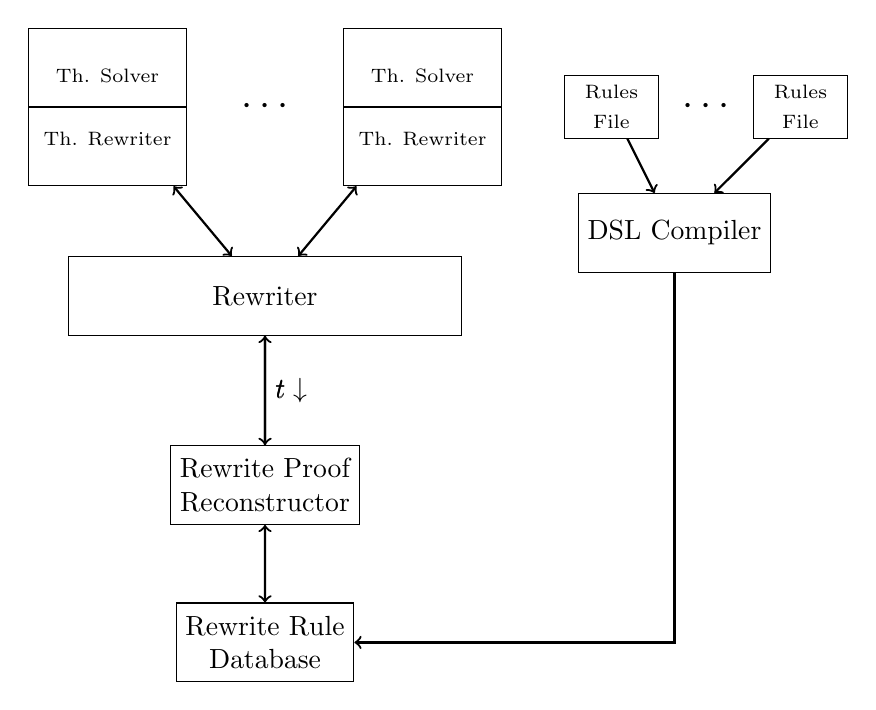
\begin{tikzpicture}[scale=0.8,
    box/.style={rectangle, draw, minimum width=2cm, minimum height=1cm, align=center, font=\normalsize},
    smallbox/.style={rectangle, draw, minimum width=1.2cm, minimum height=0.6cm, align=center, font=\small},
    arrow/.style={->, thick},
    bidirectional/.style={<->, thick}
]

% Combined Theory Solver/Rewriter boxes
\node[box, minimum height=2cm] (combined1) at (0, 5) {};
\node[box, minimum height=2cm] (combined2) at (5, 5) {};

% Add text labels
\node at (0, 5.5) {\scriptsize Th. Solver};
\node at (0, 4.5) {\scriptsize Th. Rewriter};
\node at (5, 5.5) {\scriptsize Th. Solver};
\node at (5, 4.5) {\scriptsize Th. Rewriter};

% Add horizontal dividing lines
\draw (combined1.west |- 0,5) -- (combined1.east |- 0,5);
\draw (combined2.west |- 0,5) -- (combined2.east |- 0,5);

% Dots between boxes
\node at (2.5, 5) {\Large $\cdots$};

% Main Rewriter (center)
\node[box, minimum width=5cm] (rewriter) at (2.5, 2) {Rewriter};

% Rules Files (right side)
\node[smallbox] (rules1) at (8, 5) {\scriptsize Rules\\ \scriptsize File};
\node[smallbox] (rules2) at (11, 5) {\scriptsize Rules\\\scriptsize File};

% Dots between rules
\node at (9.5, 5) {\Large $\cdots$};

% DSL Compiler
\node[box] (dsl) at (9, 3) {DSL Compiler};

% Rewrite components (bottom)
\node[box] (proof_reconstructor) at (2.5, -1) {Rewrite Proof\\Reconstructor};
\node[box] (rule_database) at (2.5, -3.5) {Rewrite Rule\\Database};

% Arrows
\draw[bidirectional] (combined1) -- (rewriter);
\draw[bidirectional] (combined2) -- (rewriter);

\draw[arrow] (rewriter) -- node[right] {$t$} (proof_reconstructor);
\draw[arrow] (proof_reconstructor) -- node[right] {$t\downarrow$} (rewriter);

\draw[bidirectional] (proof_reconstructor) -- (rule_database);

\draw[arrow] (rules1) -- (dsl);
\draw[arrow] (rules2) -- (dsl);
\draw[arrow] (dsl) |- (rule_database.east);

\end{tikzpicture}
\caption{Overview of the components of our approach}
\label{fig:system_overview}
\end{figure}

To address this problem, we use the domain-specific language RARE \cite{rare} provided by cvc5 for defining rewrite rules. As described in \cref{sec:rare-intro}, RARE elaborates proofs for specific rewrite steps on demand based on built-in rewrite rules of cvc5.
The RARE rule used and its arguments are made explicit in the \lstinline[language=SMT]{:args} parameter of the rule \kw{rare\_rewrite} in the proof trace.
cvc5 elaborates the proof by rendering each coarse step into fined grain with atomic rewrite.
Although RARE is currently only supported by cvc5, its use has allowed us to increase the success rate of proof reconstruction.

The example of \cref{lst:or_simp_example} illustrates how RARE transforms an Alethe proof trace into a more fine-grained proof.
The original step \texttt{t1} uses the rule \texttt{or\_simplify} by applying twice the transformation (2).
However, cvc5 can output instead a proof trace using RARE that indicates the rule \kw{bool-or-false} and makes the arguments explicit.
Note that the RARE format represents an empty list as \kw{rare-list} without argument.

\begin{example}[RARE example] An original step $\kw{or\_simplify}$ below
\begin{lstlisting}[language=SMT]
(step t1 (cl (= (or false x y false z) (x y z)))
      :rule or_simplify)
\end{lstlisting}

can be changed by cvc5 if RARE is enabled into:

\begin{lstlisting}[language=SMT,caption={\texttt{or\_simplify} elaborated by RARE}, label={lst:or_simp_example}]
(step t1 (cl (= (or false x y false z) (or x y false z)))
      :rule rare_rewrite :args ("bool-or-false" rare-list
                                   (rare-list (x y false z))))
(step t2 (cl (= (or x false y z) (or x y z)))
      :rule rare_rewrite :args ("bool-or-false" (rare-list x)
                                   (rare-list (y z))))
\end{lstlisting}
\end{example}


\section{Elaborating lia\_generic steps}
\label{sec:elaboration-lia}

The rule \tt{lia\_generic} is similar to \tt{la\_generic}, but omits the coefficients,
i.e.\ \colorbox{orange!30}{$[a_1 \dots a_r]$} is empty..
%Since this rule can introduce a disjunction of arbitrary linear integer inequalities without any additional hints, proof checking is \emph{NP-complete} \cite{Schrijver:lia}.
We decided to leverage the elaboration process of \tt{lia\_generic} performed by Carcara, as doing otherwise would require implementing Fourier-Motzkin elimination for integers, as done in \cite{micromega,omegatest}, hence reimplementing work that was already done by the solver.

Carcara considers $\tt{lia\_generic}$ steps as holes in the proof, given that ``their checking is as hard as solving'' \cite[\S 3.2]{carcara}.
To address this, Carcara leverages an external tool that reformulates each \tt{lia\_generic} step as a separate problem and produces Alethe proofs not containing \tt{lia\_generic} steps.
The proof is then imported and validated, replacing the original step.
%% sm: I don't see why this remark is relevant for this paper?
%However, at present, Carcara only uses the solver cvc5 for performing this task.
Thus, the step
% In detail, the elaboration method, when encountering a \tt{lia\_generic} step
%
\begin{lstlisting}[language=SMT]
    (step S (cl (not l1) ... (not ln)) :rule lia_generic)
\end{lstlisting}
%
concluding the clause $\neg l_1 \lor \dots \neg l_n$ where all $l_i$ are inequalities, generates an SMT-LIB problem asserting $l_1$, \dots, $l_n$ and invokes the solver cvc5 on it, expecting an Alethe proof $\pi : (l_1 \land \dots \land l_n) \ra \bot$
that does not use \tt{lia\_generic}. Carcara will check this subproof and then replace the original step by a proof of the form

\begin{lstlisting}[language=SMT,caption={Elaboration of \tt{lia\_generic}},label={lst:elab_lia}]
(anchor :step S.t_m+1)
(assume S.h_1 l1)
...
(assume S.h_n ln)
...
(step t.t_m (cl false) :rule ...)
(step t.t_p (cl (not l1) ... (not ln) false) :rule subproof)
(step t.t_q (cl (not false)) :rule false)
(step S (cl (not l1) ... (not ln)) :rule resolution :premises (S.t_p S.t_q))
\end{lstlisting}

% In the next section, we first present an overview of our embedding of Alethe in Lambdapi, and then our automatic procedure to reconstruct $\tt{la\_generic}$ step that appear in LIA problem.
